\documentclass[11pt,a4paper]{article}

% ---------- Packages ----------
\usepackage[margin=1in]{geometry}
\usepackage[T1]{fontenc}
\usepackage[utf8]{inputenc}
\usepackage{lmodern}
\usepackage{microtype}
\usepackage{setspace}
\usepackage{graphicx}
\usepackage{float}
\usepackage{hyperref}
\usepackage{caption}

\setstretch{1.15}
\captionsetup{font=small,labelfont=bf}
\setcounter{tocdepth}{2}

% ---------- Title ----------
\title{Intelli-Trading Fours: Interim Report}
\author{Emmanuel Areoye}
\date{22/12/2025}

\begin{document}
% =====================================================
% Cover Page
% =====================================================

\begin{titlepage}
    \centering
    \vspace*{3cm}

    {\Large\bfseries Intelli-Trading Fours\par}
    \vspace{0.5cm}
    {\large An AI-Driven Rhythmic Improvisation System\par}

    \vspace{2.5cm}

    {\large Interim Project Report\par}
    \vspace{0.5cm}

    {\large BSc Computer Science\par}
    \vspace{0.25cm}
    {\large University of Nottingham\par}

    \vspace{2cm}

    {\large Module: Individual Project / Dissertation\par}
    \vspace{0.25cm}
    {\large Academic Year: 2024--2025\par}

    \vspace{2cm}

    {\large Student Name: Emmanuel Areoye\par}
    \vspace{0.25cm}
    {\large Student ID: PSYEA6\par}

    \vfill

    {\large Supervisor: Juan Martinez Avila\par}
    \vspace{0.5cm}
    {\large \today\par}
\end{titlepage}


\pagenumbering{arabic}
\setcounter{page}{1}

\maketitle
\vspace{-1.2em}

% =====================================================

% =====================================================
% Table of Contents
% =====================================================

\tableofcontents
\newpage

\section*{Abstract}
This interim report presents the progress of the Intelli-Trading Fours project, an AI-
driven rhythmic improvisation system inspired by the jazz practice of trading fours. The
project explores real-time human-AI musical collaboration using a combination of Unity,
ChucK, and percussion input. This report outlines the motivation for the project, reviews relevant literature in musical metacreation and machine musicianship, describes the system architecture and current implementation, discusses preliminary testing results, and reflects planned future development activities.

% =====================================================
\section{Introduction}

\subsection{Design Brief}
The increased adoption of Artificial Intelligence has expanded past traditional analytical and optimisation-based domains, extending into creative systems with the purpose of augmenting and collaborating with human artistic expression. Within music, this phenomenon has motivated the development of computational systems not only to attempt autonomous generation of musical material but also seek to meaningfully interact with human performers.

The design brief for this project is to address the challenge of facilitating real-time, musically and rhythmically adept human-AI musical collaboration. Specifically, this project aims to explore how an artificial agent can musically respond and participate with a human performer in an improvisational exchange that emphasises listening, timing and dialogue as opposed to pre-generated output.

\subsection{Motivation}
The motivation for Intelli-Trading Fours takes inspiration from the improvisational practice in Jazz known as “trading-fours”: when musicians alternate short improvised phrases in a conversational manner. This practice demands strong collaboration and near-instant responsive creativity. Research across different interdisciplinary papers show that interactive improvisation engages distinct cognitive and neural processes, reaffirming this project’s emphasis on mutual responsiveness and temporal alignment when approaching music creation (Donnay et al., 2014).

This is particularly pertinent to human-AI musical collaboration as it presents a compelling and dynamic interaction model. The system will follow an enforced turn-taking structure, requiring temporal alignment and mutual responsiveness, thus serving as an examination of how artificial agents function as a true musical partner. These principles will be embedded into a computational system that supports rhythmic dialogue between a drummer and an AI agent.

\subsection{Background and Context}
The increased uptake in creative AI has given rise to the field of Musical Metacreation (MuMe): an exploration in computational systems’ participation in musical tasks such as composition, performance and improvisation. Contemporary research explores interactivity and co-creation within these systems where both human and computational agents engage in musical dialogue (Pasquier et al., 2016).

The challenge presented is illustrated by the dichotomy between the multifaceted nature of humans perceiving rhythm and machines’ reliance on tangible structure and order. Musical rhythm is inherently temporal and dependent on structures, yet human perception of rhythm entails complex cognitive mechanisms like entrainment (Levitin, Grahn \& London, 2018). The combination of structural regularity with perceptual variability complicates attempts to formalise rhythm within computational systems.

Existing AI musical agents have demonstrated varying degrees of success in generative capability and stylistic imitation however these applications often prioritise autonomous output or offline generation, with few prioritising real-time, turn-based improvisational exchange between the two players (Pachet, 2002). This gap provides the contextual relevance for this project.

\subsection{Project Overview}
The aim of this project is to design and implement a real-time AI drumming system with the ability to listen to and improvise on a performer’s rhythmic input. The system is developed using Chunity, a programming environment that can combine ChucK’s sample-accurate timing with Unity’s visual and interactive capabilities. Rhythmic performance is captured from an electronic percussion interface and processed in an interactive turn-based workflow. The workflow is an interactive turn-based exchange and the AI agent is explicitly positioned as a responsive partner to explore how latency, timing accuracy and rhythmic representation influence the quality of HCI.
% =====================================================
\section{Literature Review}

\subsection{Musical Metacreation and Machine Musicianship}
Early and contemporary systems vary in how machine creativity is conceptualised from autonomous generative composers to interactive agents dependent upon a live musical dialogue. These approaches can be examined across three conceptual axes: 
autonomy versus co-creativity
product-centred versus process-centred creativity
determinism versus emergence in creative systems

\subsubsection{Autonomous Creativity vs Co-Creative Systems}
This axis is not about whether collaboration exists but where agency is situated and whether the system is responsive to human musical interaction in real-time.

Musebots are a class of autonomous musical agents designed to generate music collaboratively with other software agents. While this system emphasises collaboration between agents, it remains confined to the system, assigning creative agency entirely to the system (Eigenfeldt 2016). 

In contrast, Pachet’s Continuator explicitly situates creativity within real-time HCI. The system is an interactive instrument that learns stylistic material from a performer and directly responds with continuations to ongoing musical user input. Creativity is shared temporally between collaborators where the creation of music emerges through bidirectional dialogue where the AI agent serves as a collaborator whose behaviour is contingent on human performance (Pachet, 2002).

The tension lies within black-box music generation versus interactive dialogue. The former prioritises output quality and its evaluation is often the result of stylistic analysis whereas the latter focuses more on the experiential quality framing musical creativity as an enactment rather than a product. 

This project explicitly rejects autonomy first-creativity in favour of a dialogical model. The main focus is not to demonstrate independent musical authorship but rather to facilitate a turn-based, responsive exchange in which musical creativity emerges collaboratively. Authorship is distributed and the creative value lies in the interaction rather than just the final output.

\subsubsection{Product-Centred vs Process-Centred Creativity}
Product-centred approaches arbitrate success based on the quality of the resulting musical artefact. This perspective suits generative composition systems where the artefact is self-contained and evaluated independently of its creative context. However, it implicitly assumes creativity is decoupled from interaction and often abstracts away temporal, performative and embodied aspects of (especially live) music making. 

Process-centred creativity brings the dynamics of interaction between human and system to the fore, it assesses the effectiveness of the system in supporting a performance. Creativity is positioned as something enacted over time based on mutual influence from each collaborator where experiential metrics are prioritised. 

Smith illustrates how interactivity in generative systems can replicate musical output yet elicit a difference in the user’s perception of collaboration and creativity. Whilst output quality served as a control variable, the independent variables of interaction design and overall system behaviour resulted in distinct creative experiences for performers, highlighting the exclusive consideration of artefact based metrics’ failure to capture key dimensions of musical creativity (Smith, 2022) further demonstrating the importance of process-centred evaluation.

This distinction is pertinent in improvisational contexts, where musical meaning unfolds moment-to-moment rather than retrospectively. It privileges temporal awareness, shared musical understanding and responsiveness, none of which take enough credence when assessed through independent static artefacts. Therefore, a process-centred approach provides a more appropriate framework for evaluating real-time interactive musical systems.

This framing bears relevance to the design and evaluation of Intelli-Trading Fours, whose trading fours Jazz inspiration treats creativity as an interactive temporal process not a fixed musical outcome. The system is not intended to optimise rhythmic artefacts assessed offline over a sustained responsive, turn-based dialogue with a performer. 

\subsubsection{Determinism vs Emergence in Creative Systems}
The balance between determinism and emergence forms the final axis in MuMe. Deterministic approaches rely upon explicitly defined rules to inform musical behaviour, privileging control and predictability over system output. However, a rigid application of these strategies risks repetitive and undynamic behaviour, outcomes unbecoming of a system intended for improvisational dialogue and expressive variation.

An emergent approach allows room for musical structure to dynamically manifest through interaction, exploiting learning-based or probabilistic functions to generate novelty. The priority given to adaptation enables responses that are not prescribed before execution. However, in a time-sensitive musical context an unconstrained emergence approach introduces the risk of instability. 

Work into early computer-aided musical composition challenges the binary consideration of determinism and emergence. Vaggione argues that reducing determinism to total predictability whilst regarding emergence as the extreme counterpart that solely begets unstructured randomness mischaracterises multi-levelled musical timing, presenting it as a single formal dimension. Early approaches often suppressed singular musical events, opting for uniform behaviour at the expense of interaction across temporal levels by relying on stochastic or deterministic global laws (Vaggione, 1993). 

Vaggione instead proposed the idea that meaningful musical structures manifested through interaction across multiple levels of temporal organisation such that constraints served as facilitators for judicious musical articulation instead of fixed prescriptions. This positions emergence as the outcome of dynamic interplay between variation and constraint. When interactions occur between local events and global form, meaningful musical coherence emerges (Vaggione, 1993). 

This balance is critical in interactive, improvisational systems that require flexibility to support expression and variation within the structured constraints. An overreliance on determinism flattens interaction with the system whilst too much emergence risks disruptive musical flow and temporal misalignment.

Intelli-Trading Fours is underpinned by this balance. The system employs determinism to enforce temporal and turn-based consistency whilst encouraging emergent musical dialogue with room to vary across successive exchanges. HCI interactions help  inform improvisation without conceding to fully deterministic behaviour or a lack of musical constraint, positioning musical creativity as a result of multi-level temporal interaction.

\subsection{AI Musical Agents and Improvisation}

\subsubsection{Reactive vs Generative Improvisation}
Rather than being solely distinguishable by generative capacity, the degree to which a system’s musical output serves as an immediate response to performer input informs the classification of a system. Conversely, how output is derived from internal generative processes over longer musical timescales also serve as an arbitrator that defines these systems.

These distinctions underline the role of temporal coupling, decision-making and overall responsiveness in improvisational agent behaviour.

Early research into interactive work framed the computer as an ensemble participant able to adjust to performance conditions instead of a “tape machine” executing preauthored material. Baird, Blevins, and Zahler introduce the idea of an “interactive computer performer” whose task is to listen to a live performer whilst noting their position within the score with the ability to adjust its own dynamics and tempo to maintain pace, reflecting the adaptive behaviour of human ensemble playing. This improvisational technique positions musical intelligence functionally as behavioural alignment with human timing and interpretive variation in an interactive setting, rather than complex generative functions (Baird et al., 1993).

Pachet’s Continuator is an exemplification of this behavioural framing, presented as a hybrid of stylistic-conscious and consistent generation with real-time musical interaction. Systems are classified as interactive or imitative and are presented such that the former tends to lack memory and style by prioritising quick input translation, whilst the latter can model style but does not support interaction. Pachet instead argued that a seamlessly integrated instrument-like agent should consider the performer’s playing mode and adapt quickly to changes in musical behaviour. In doing so, Continuator demonstrates how longer-term musical structure can be implemented into live improvisation without compromising temporal coupling; all in all illustrating the balance between moment-to-moment reactivity and generative continuity (Pachet, 2002).

More recent work positions these requirements as even more critical in embodied improvisational contexts. Hoffman and Weinberg’s robotic marimba player Shimon is characterised with the ability to improvise in real-time while listening to and building upon a pianist’s performance. This research explicitly attributes the success of joint improvisation to factors such as communicative physical cues, anticipatory action and synchronisation because faults in these areas are immediately perceivable. Their studies reinforce the idea that coordination and perceived responsiveness are contingent on embodiment and visual contact - ratifying the idea that improvisation is deemed credible within the quality of interaction rather than output alone (Hoffman and Weinberg, 2011). 

A system with an aversion to reactivity can result in output too congruent with the user’s original input whilst one that overprioritises autonomy can become too musically incongruent to be deemed an improvisation of the original input; this suggests improvisation needs to leverage hybrid behaviour. 

Trading fours’ meaningfulness emerges through temporally bounded, alternate and responsive collaboration and Intelli-Trading Fours adheres to these principles by seeking to strike a suitable balance of reactive and generative musical creation.

\subsubsection{Temporal Scope and Musical Continuity}
Some systems make decisions based on short term musical information, reacting to recent events while others incorporate longer representations of musical attributes such as style, form and structure. 

A system with a short term temporal scope means more of a focus on local music continuity. Rapid adaptation and tight temporal coupling are facilitated through decision making based on rhythmic patterns, recent phrases or immediate performer behaviour. This follows a model of interactive music systems in which real-time listening and reaction from higher level structures have a higher degree of separation, allowing agents to react to more minute or instant musical changes (Rowe, 1991). 

Alternatively, systems that operate using a longer temporal scope retain musical representations accumulated across extended periods. The representations may include learned structure, encoded stylistic features or higher level musical expectations, these allow output generated by the system to imply a grasp of coherence. However, increased reliance on this approach can compromise the reactiveness of the system in regards to the local musical context, especially if weighting of these global representations are much stronger than the real-time decision making. Studies in rhythmic modelling demonstrate that systems designed with this bias can trade off immediate adaptability, resulting in an outputted response that is less sensitive to local temporal variation (Gillick et al., 2019). 

With regards to improvisation, long term temporal scope introduces a tension between continuity and control; agents that heavily rely on prior musical knowledge may begin to steer interactions towards inadvertently predefined avenues rather than fluidly complementing the human input. This undermines improvisation as a collaborative dialogue, especially in the context of turn-based musical creation. 

Hybrid approaches serve as attempts to rectify these tensions by stratifying the temporal process. This decoupled approach means long term representation broadly influences stylistic tendencies not necessarily immediate output whereas short term functions handle aspects regarding alignment with the performer. This separation serves as a means to maintain and balance musical coherence with interactional sensitivity in real-time (Rowe, 1991). 

In this project, Intelli-Trading Fours defines long term musical memory as explicitly constrained to allow musical continuity through alternation and response rather than excessive internal planning because the long term representations risk conflicting with interactional logic, whereas short term mechanisms can support responsive dialogue whilst still maintaining coherence rhythmically. 

\subsection{Rhythm-Based Human--AI Interaction}
Rhythmic information is perceived continuously not retrospectively like melody or harmony, this short temporal nature allows performers to respond to timing deviations as they occur. This is substantiated by findings in music psychology that link rhythmic perception directly to motor coordination, positioning rhythm as the primary interface between perception and action (Levitin et al., 2018). 

Research in music cognition shows humans to be highly sensitive to temporal variation, with minute changes in timing demonstrating intention and interactional awareness. Rhythmic synchronisation and entrainment are intrinsically linked in collaborative performance; it allows musicians to communicate without explicit signalling. Studies in interactive improvisation, including studies explicitly about trading fours, illustrate temporal alignment’s role in underpinning shared musical understanding during performance (Donnay et al., 2014). 

In an improvisational context, rhythm functions as both an affordance and a constraint. Temporal regularity supports coordination by acting as a shared reference framework, of which deviations facilitate collaborative expression. Rhythmic interaction only needs timing to allow meaningful exchange. Performance and ethnomusicological studies of Jazz improvisation preposition rhythm as necessity for musical interplay, where there exists a negotiation of interaction through timing (Hodson, 2007).

\subsubsection{Entrainment, Timing, and Mutual Adaptation}
Entrainment is the process through which performers can dynamically adjust their timing to achieve mutuality. Instead of a fixed temporal reference, timings can be the result of microvariations that are adapted to by musicians, resulting in a dynamic shared temporal framework during a performance. Timing itself becomes the communicative medium that allows rhythmic interaction to act as a form of dialogue.

Studies of collaborative human improvisation present entrainment as reciprocal. The mutual adaptation of timing allows performers to maintain coordination while preserving expressive freedom, further positioning improvisation as a collective process. Neuroimaging studies of jazz musicians engaged in trading fours illustrate the practice relies on predictive timing and active listening (Limb \& Braun, 2008).

Entrainment presents an essential design challenge in HCI - systems need to be able to adapt their timing based on human input while retaining the stability to perceive the rhythm itself. Rigid timing suppresses expressive interaction and excessive flexibility induces temporal misalignment. Successful improvisational systems therefore require functionality that allow mutual temporal adaptation and don’t impose a preferred synchronisation. 

\subsubsection{Turn-Taking and Trading Fours as Musical Dialogue}
Turn taking is the structured framework where rhythmic improvisation acts as dialogue instead of simultaneous performance. It foregrounds listen and response with alternation that has explicit boundaries between reception and contribution. In this way, temporal and expressive space isn’t fought over, instead agency is evenly distributed. Trading fours is the exemplification of this dialogic structure in Jazz improvisation. Performers alternate between leading and responding roles along fixed temporal segments (Donnay et al., 2014).  Stacked contributions and the relations they share with each other convey musical meaning which is why Jazz scholarship deems this process conversational (Hodson, 2007).

Since transition points are negotiated instead of simultaneity, trading fours is particularly suitable as a model for a HCI as the system is not required to explicitly infer human intention and can instead rely on clearly defined triggers that indicate action and response moments. For an interactive musical system, alternation removes ambiguity as agency becomes shared and derivable. Intelli-Trading Fours deliberately adopts this structure in alignment with an established improvisational practice to function not only as musical inspiration but as an interactional framework for balanced human-AI rhythmic dialogue.

% =====================================================
\section{System Design}

\subsection{System Architecture Overview}
Figure 1 presents the high level system architecture. It is a distributed interactive music pipeline that transforms physical percussive performance into symbolic rhythmic representations used to generate a complementary improvisation. Sensing, interaction logic and audio rendering are deliberately decoupled which facilitates the optimisation of each layer independently while preserving a clear interpretable data flow between them. 

Interaction begins with a human performer playing a beat on a drum pad fit with a Piezo Disk that connects to Bela - which performs sensor sampling and forms the embedded instrument layer. Hits are encoded into control messages containing: an instrument identifier, a velocity value and timing information. These events are transmitted as a symbolic event to the host system using Open Sound Control (OSC) - a protocol deliberately chosen for its low latency and widespread adoption in digital musical instruments. This creates an explicit boundary between physical sensing and higher-level musical reasoning and completes the control message exchange.

The symbolic event stream is received by an IMPS style interaction engine running on the host system. This term IMPS style is used to indicate the conceptual alignment with existing interactive music prediction systems that frame musical interaction as the real-time processing of control streams,  rather than to imply direct use of the IMPS system or its MDRNN-based prediction architecture (Martin and Torresen, 2019). 

The interaction engine encapsulates three tightly coupled responsibilities: 
Incoming hit events are converted into an internal rhythmic representation deliberately designed for computational transformation. 
The engine manages the temporal structure of interaction which includes alternation between human and machine 
It uses a responsive transformation model that outputs generated machine responses. 
The model is conditioned on recently captured human material, facilitating continuity and a perceptible musical dialogue. 

The system derives its responses through motif preserving variation with complementary constraint application. The resulting response is then encoded into the uniform symbolic rhythmic pattern before being passed downstream for playback. 

Audio rendering is handled by a dedicated playback engine implemented leveraging ChucK and integrated into Unity via Chunity. The interaction engine transmits symbolic response patterns to the audio layer which schedules events relative to the system’s timing model before rendering them as sound output. The specialised engine’s delegation of scheduling and audio synthesis ensures the system avoids conflating interaction logic with low level audio concerns, optimising conceptual clarity and system reliability.

The relationship between interaction structure and musical timing is a critical consideration in this architecture. While the practice of trading fours traditionally assumes metrically defined turns, drum pad interaction may exhibit weakly defined time signatures or loose and unconventional timing. To mitigate the effects of this, interaction is currently structured around temporal segments with audibly communicated fixed lengths. These segments are aligned to a metrical grid providing a robust framework for alternation and response generation. Notwithstanding, the architecture leaves room for extension in regards to alternative segmentation strategies such as time-based windows or adaptive segmentation length functionality in the event that metrically constrained interaction becomes surplus to requirement. The current implementation of the timing model  and alternation logic as they stand are elaborated in later sections of Chapter 3.

All in all, Figure 1 supports real-time, turn-based rhythmic interaction through explicit decoupling of physical sensing, symbolic interaction logic, and audio rendering. The pipeline's modularity not only supports the implementation of the baseline system but presents the opportunity for future experimentation with regards to submodules such as the timing models and response generators without disturbing the peripheral interaction framework. 

\begin{figure}[H]
  \centering
  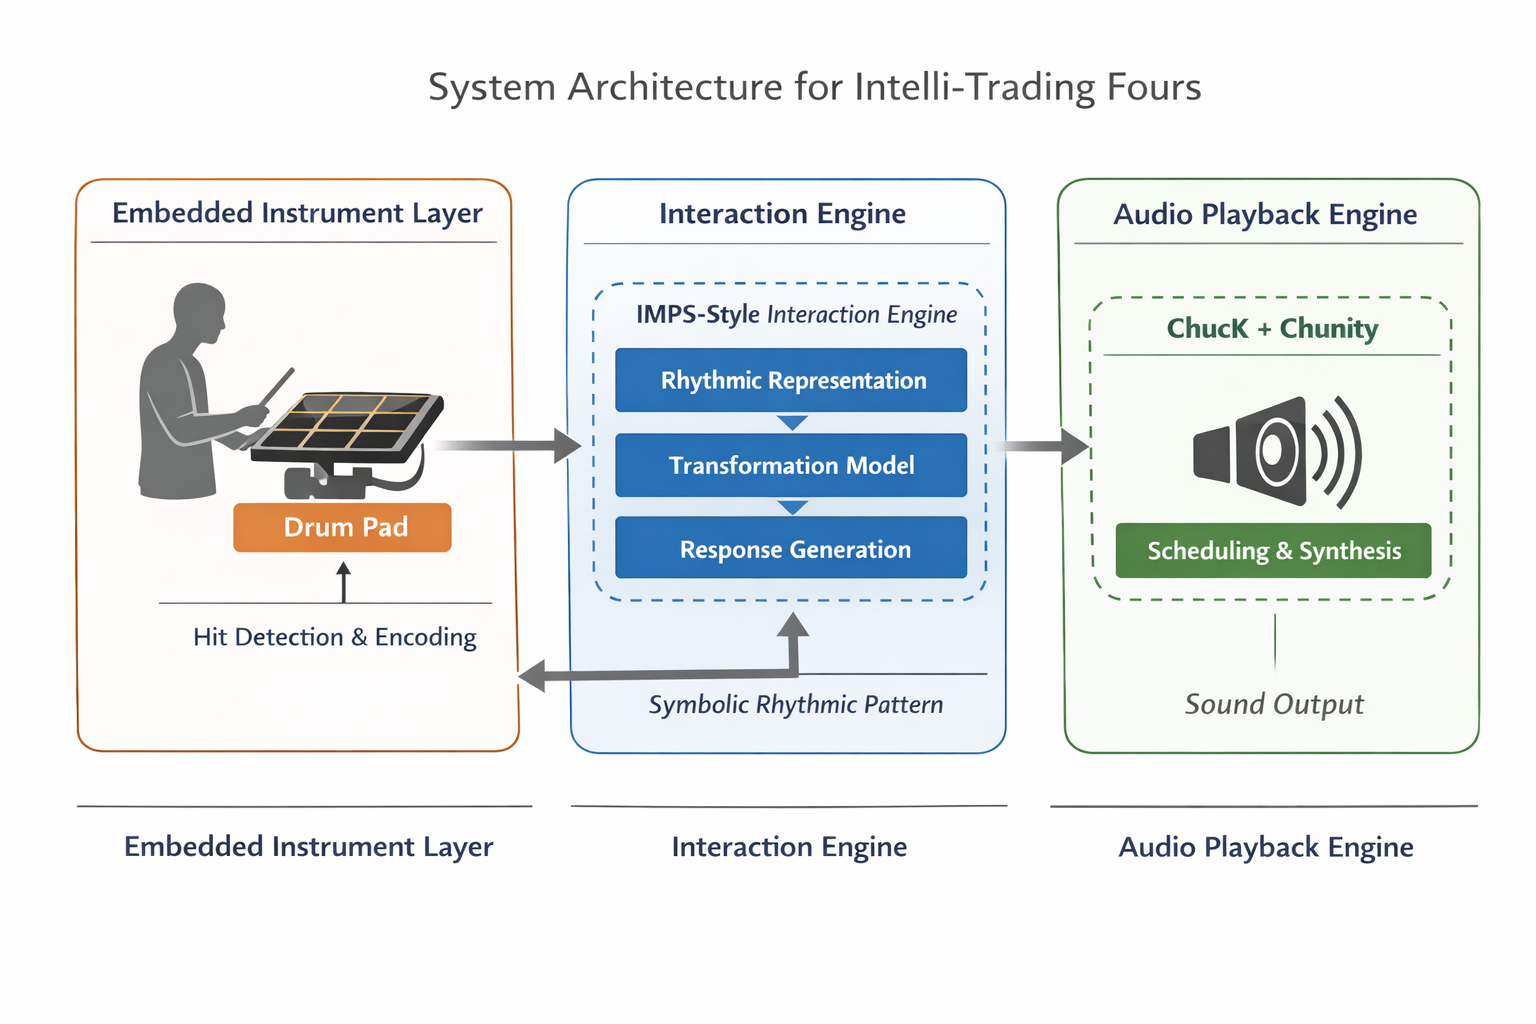
\includegraphics[width=\linewidth]{figures/System Architecture (interim).png}
  \caption{System Architecture for Intelli-Trading Fours}
  \label{fig:system_architecture}
\end{figure}

\subsection{Timing Model and Synchronisation}
The timing model of Intelli-Trading Fours is critical as rhythmic interaction is contingent on what is played but also when its playback is scheduled to occur. Unlike music systems operating with fixed score representations, drum pad performances can produce temporally ununiform control data that may include uneven spaces between events and weakly defined time signatures. The design of this model must reconcile the need for stable interaction under time constraints that also support the proposed interaction structure.

The nature of drum pad percussion doesn’t inherently entail metrical structure. While the performer may have an internal metronome, this is not empirical, especially under the context of improvisation. Therefore, imposing rigid quantisation could undermine expressive intent.

In addition, Intelli-Trading Fours operates as a distributed system with the separation of concerns between sensing on embedded instrument layer and interaction logic executed on the host system. This introduces a potential source of latency that needs to be accounted for at the symbolic representation level.This informs the timing model’s design such that it can tolerate human imprecision while still maintaining the essence of the interaction framework.

The host system maintains ownership of the interaction clock and defines temporal segment boundaries such that turn transitions occur when the segment expires, disabling input capture and triggering response generation.


\begin{figure}[H]
  \centering
  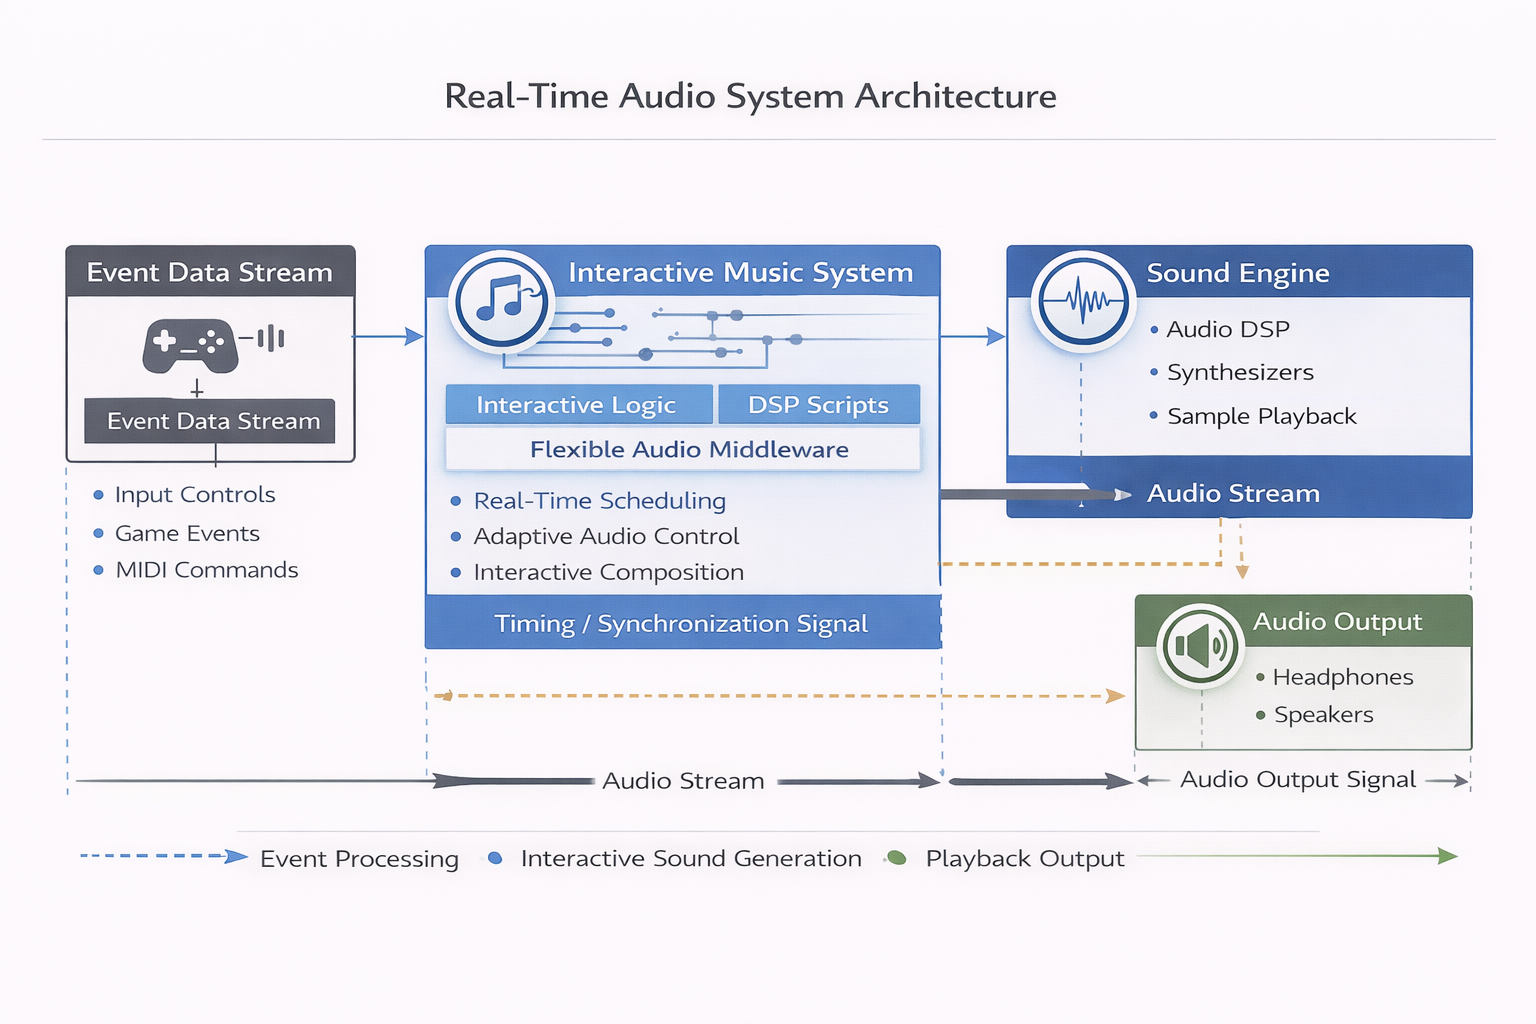
\includegraphics[width=\linewidth]{figures/Real-Time Audio System Architecture.png}
  \caption{High-level real-time audio system architecture showing event flow, interaction logic, and audio rendering.}
  \label{fig:audio_system_architecture}
\end{figure}


\subsection{Responsive Transformation Model}
The response generation module is designed to produce machine performed rhythmic percussion that is perceivably derived from percussive input and musically complementary. Response generation is not treated as the synthesis of independently derived rhythmic patterns but frames interaction as a transformation problem: given a stream of human input, the machine responds with a relevant, structured output of percussive material. 

This framing is conceptually aligned with the Interactive Musical Prediction System (IMPS), which models musical interaction as the real-time processing of embodied control streams, while explicitly diverging in both implementation and representation (Martin and Torresen, 2019).

\begin{figure}[H]
  \centering
  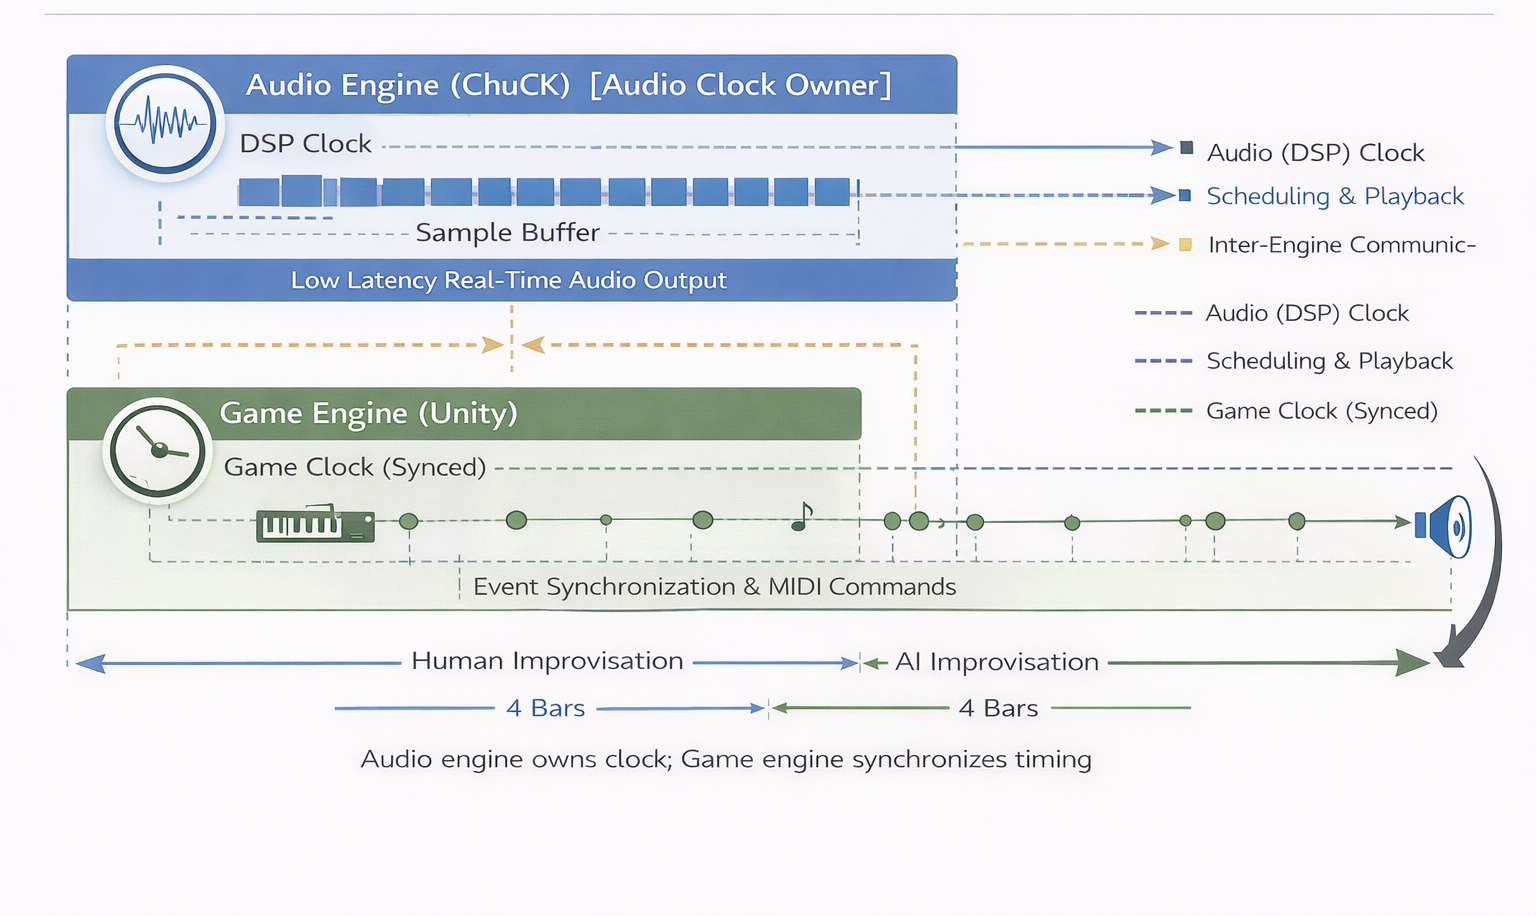
\includegraphics[width=\linewidth]{figures/Timing & Synchronisation Diagram (Interim).png}
  \caption{Real Time Audio Clock Synchronisation}
  \label{fig:timing_sync}
\end{figure}

\subsubsection{Prediction versus Transformation}
Response behaviour can be classified as either predictive or transformational. Predictive systems attempt to estimate a performer’s next action, often by modelling temporal sequences of control data, transformational systems produce variations derived directly from captured input (Rowe, 1993; Lewis, 2000). 
Intelli-Trading Fours’ alternation structure features explicit temporal boundaries on interaction, rendering IMPSs continuation less appropriate than bounded response generation. Producing a complementary rhythm requires deviation from strict continuation to prioritise dynamic variations such as: contrasting densities, filling temporal gaps or redistributing percussive emphasis. As such, the system treats human input as the conditioning context as opposed to a sequence to be directly extrapolated.

\subsubsection{Input Representation and Conditioning Context}
The response generator operates on rhythm representations from the performer's most recent interaction sequence. The representation consists of encoded events, pad identity and relative timing information. A set of contextual features is also derived to ascertain the characteristics like repetition, motif strength that can inform transformation.
This mirrors the functional role of hidden state representations within RNNs while retaining interpretability and control over the system’s behaviour.

\subsubsection{Two-Stage Response Generation Process}
Motif preservation produces an altered representation by applying controlled transformations to the performer's input pattern. They’re deliberately designed to retain perceptible rhythmic motifs while introducing variation. For example, adding or removing events in sparse or dense regions, shifting the position of repeated subpatterns and ornamenting existing. The degree of variation applied at this stage is parameterised such that divergence can be explicitly tuned through  variation strength, density scaling, and emphasis bias, which control the similarity-contrast trade-off.

It is then filtered through complementary constraints to ensure the improvisation offers sufficient musical support like tuning beat distribution, temporal emphasis and bar level congruence. Additional constraints are imposed to maintain musical plausibility and prevent exploitative model behaviour such as repetitive output or excessive simultaneity. 

This two-stage design avoids two common failures in interactive improvisation systems: direct imitation, which can quickly become repetitive and undermine performer agency, and unconstrained generation, which risks producing responses lacking stylistic coherence or perceptible relation to the input (Rowe, 1993; Lewis, 2000; Wiggins, 2006). By structuring response generation as constrained transformation, the system maintains recognisable progression from the performer’s material while retaining musical agency for both performers (Pachet, 2006; Eigenfeldt, 2016).

\begin{figure}[H]
  \centering
  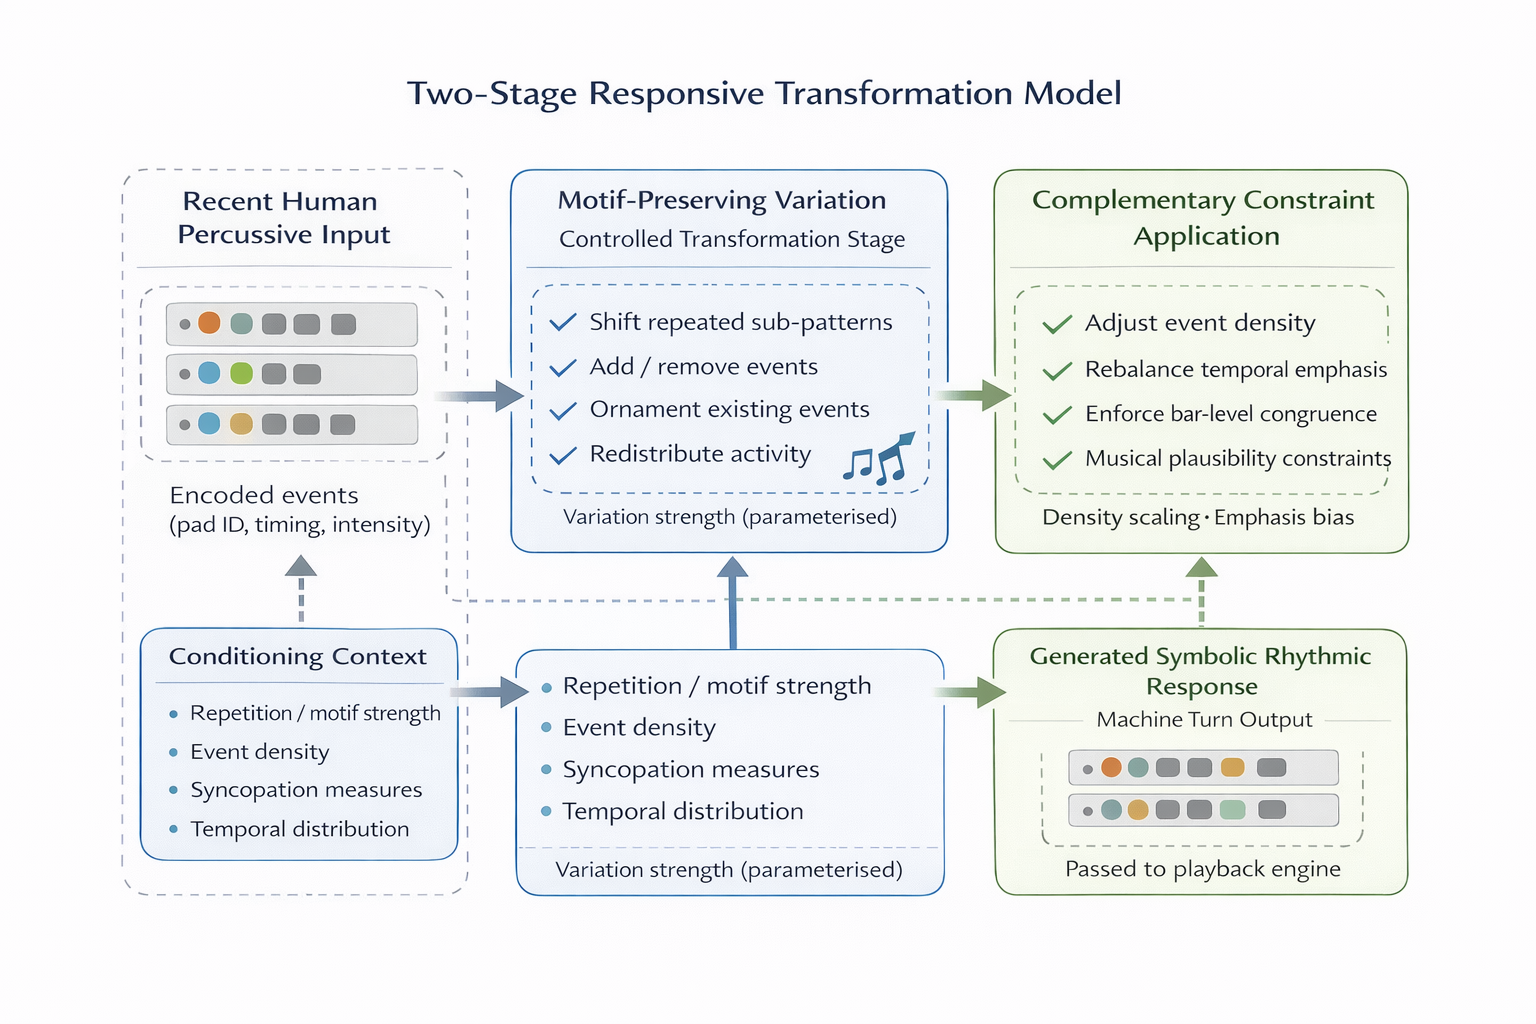
\includegraphics[width=\linewidth]{figures/Two-stage responsive model flowchart.png}
  \caption{Two-stage responsive transformation model.}
  \label{fig:two_stage_model}
\end{figure}

\subsubsection{Relation to Learning-Based Models}
The baseline system does not leverage explicit model training; however its structure deliberately emulates a learning based approach. The representation data can be incorporated into sequence based or probabilistic models such as Markov models or RNNs to ascertain nonlinear relationships between rhythmic features and response behaviour. The design leverages underlying relationships within the data that would otherwise be ascertained by predictive models.

This positions the response generator as a deliberate pragmatic compromise that seeks to optimise both expressive musical generation and implementation tractability. Despite the agility of IMPS in generating new material under time constraints, the preliminary requirements are relatively exhaustive (Martin and Torresen, 2019). By contrast, the present approach favours interpretability and responsiveness within a manageable yet scalable interaction framework.

\subsubsection{Output and Integration with Playback}
The result of the response generator is a symbolic rhythmic pattern compatible with the system’s playback engine.The pattern is rendered during the machine's turn, completing the call and response loop and maintaining consistency between interaction logic and audio realisation.

\begin{figure}[H]
  \centering
  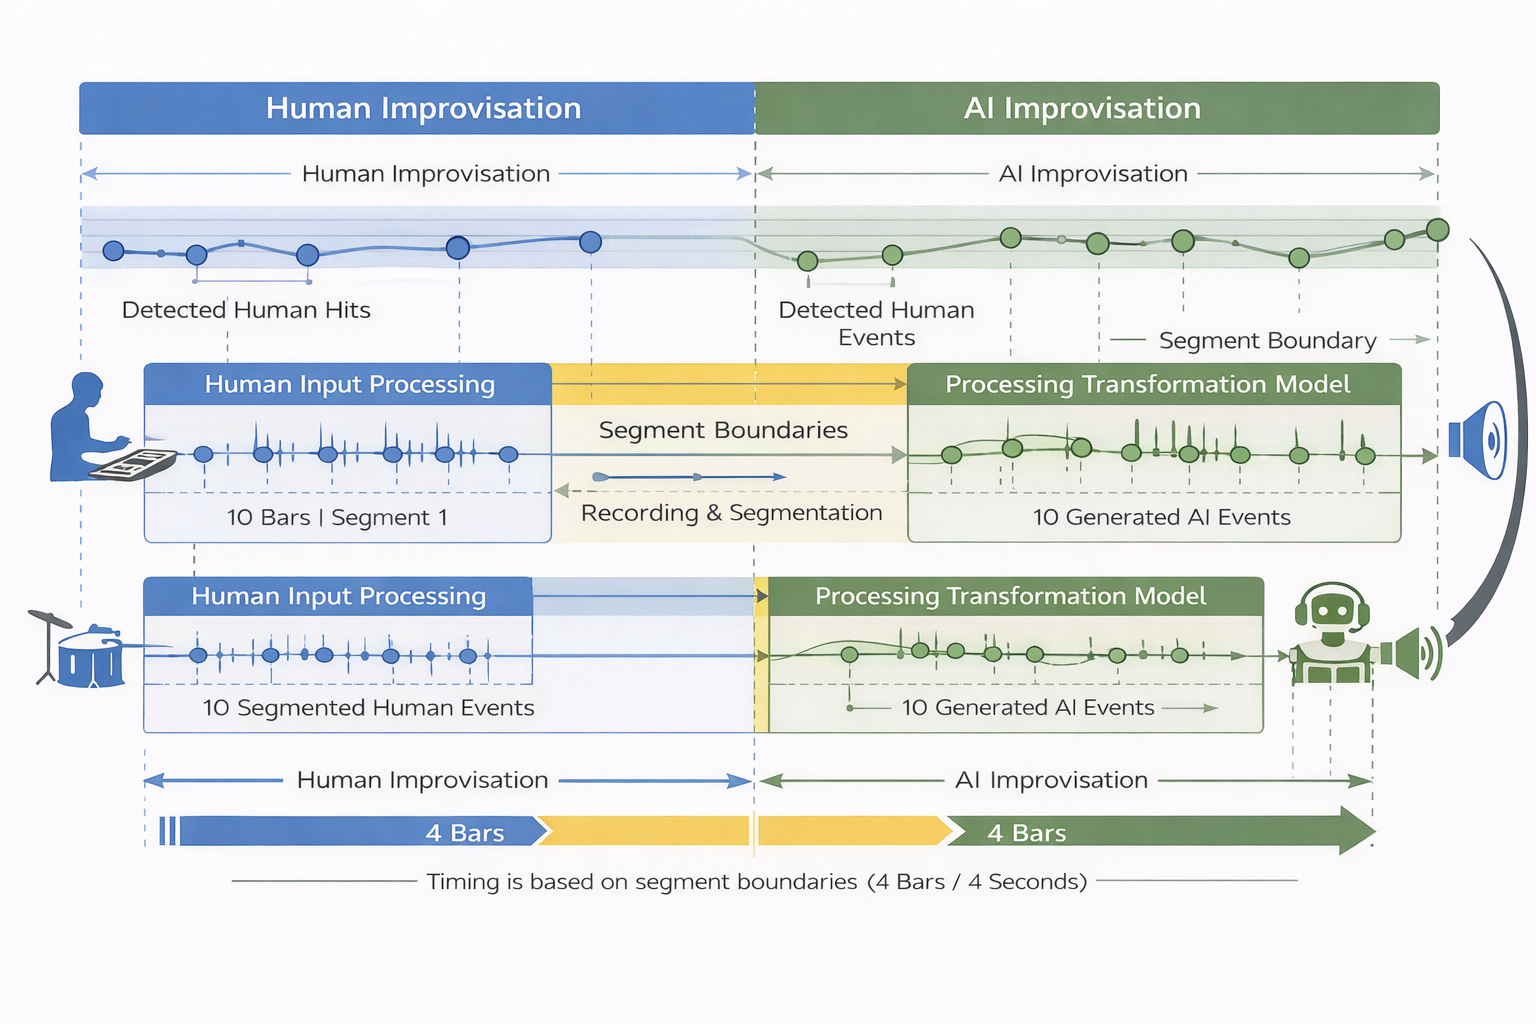
\includegraphics[width=\linewidth]{figures/Interaction Timeline Diagram (Interim).png}
  \caption{Interaction timeline showing alternating human and AI improvisation segments.}
  \label{fig:interaction_timeline}
\end{figure}

% =====================================================
\section{Interim Progress and Planning}

\subsection{Current Implementation Status}
Implementation thus far has concentrated on developing and validating the technical infrastructure needed for a real-time rhythmic interaction in Chunity. Early work established basic feasibility by embedding ChucK scoped execution within Unity and confirming reliable audio output, before progressing to a file-based execution model that supports persistent ChucK programs in Unity scenes.

The main prototype consolidates this functionality within a dedicated Unity controller that launches a combined ChucK script and manages runtime communication. Sanity checks and a readiness handshake is implemented such that Unity polls a ChucK initialisation flag before broadcasting any events, ensuring ChucK shreds and listeners are fully initialised before any interaction. This is followed by an explicit clock synchronisation phase where Unity transmits its own internal timestamp and waits for confirmation that clocks have been mapped successfully. To improve robustness, this logic includes safeguards against duplicate requests and race conditions during callback handling.

Interaction testing is supported through Unity-driven broadcast events for drum triggers that pertain to different elements of a drumkit alongside prototype control for one-bar recording and playback. Through these features, a controlled environment for exercising Chunity’s tolerance for rhythmic I/O is enabled. Timing instrumentation is also developed by transmitting per-hit Unity timestamps to ChucK, enabling comparative investigation into scheduled Unity audio times and ChucK’s internal event system. This testing allowed latency and jitter to be observed and analysed empirically rather than inferred. 

Overall, the current implementation demonstrates stable Chunity integration and reliable event-based communication and a functioning timing comparison mechanism. These findings validate the feasibility of the proposed system and surface practical constraints around synchronisation and temporal rigidity that inform subsequent design choices. 

\begin{figure}[H]
  \centering
  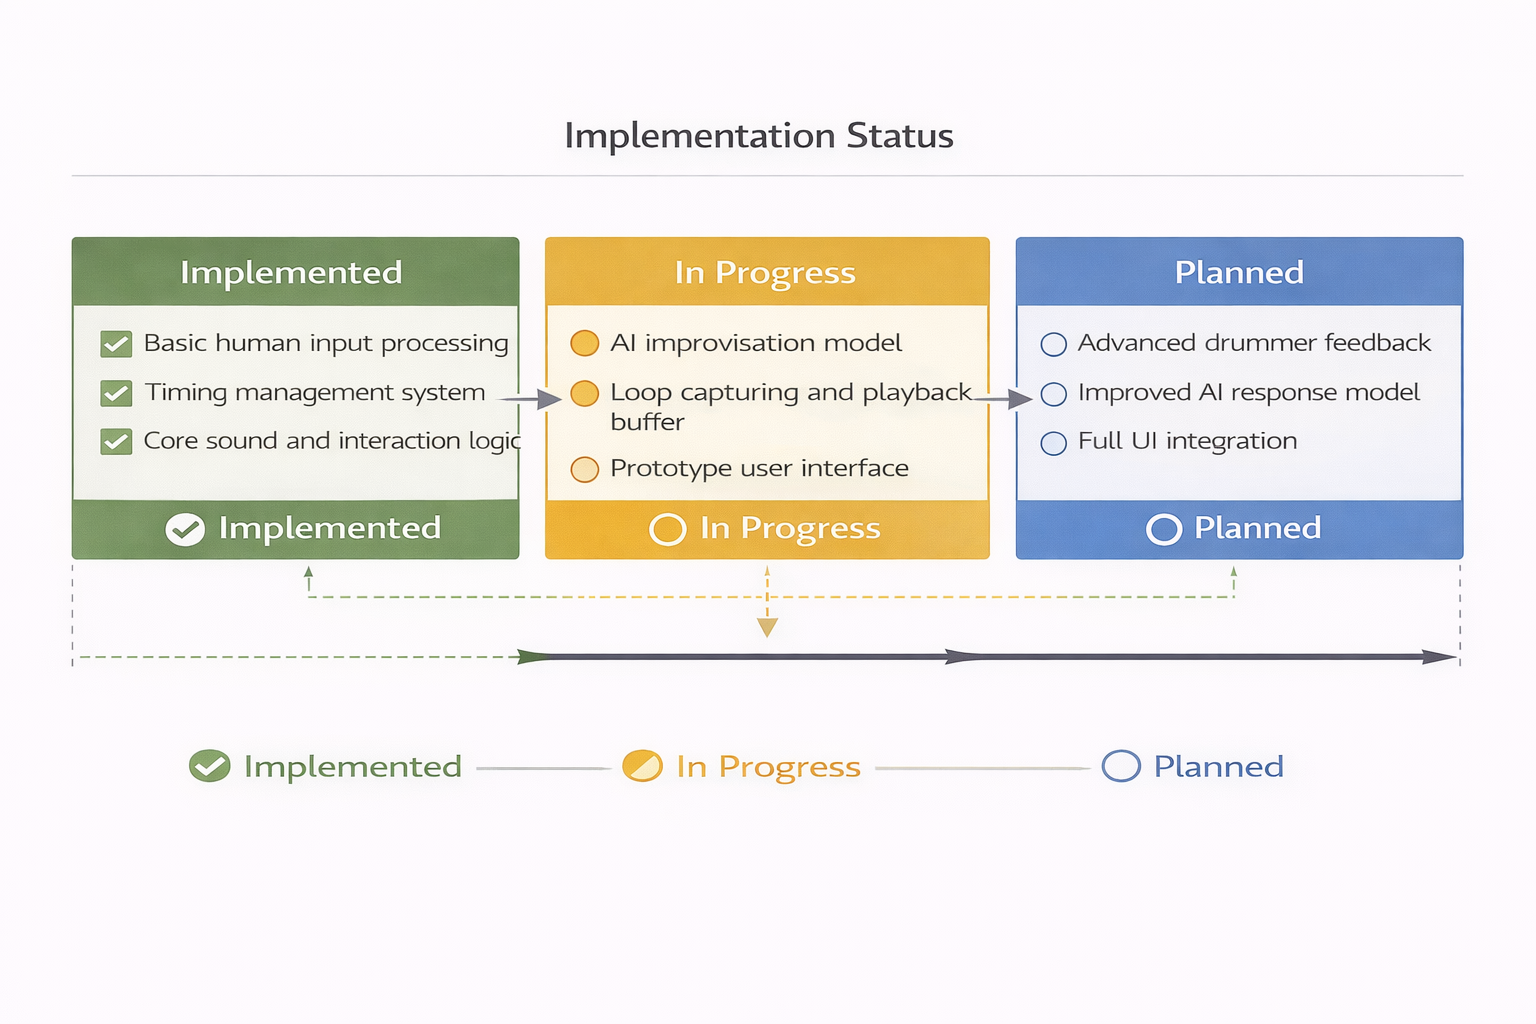
\includegraphics[width=\linewidth]{figures/Software project implementation status flowchart (Interim).png}
  \caption{Implementation status at interim stage.}
  \label{fig:implementation_status}
\end{figure}

\subsection{Research Scope and Contribution}
The project scope at this interim stage is deliberately focused on establishing and validating the technical foundations necessary to produce what my design brief states, rather than delivering a complete trading fours gameplay system. The work completed to date prioritises time infrastructure, Chunity communication and rhythmic event handling - the necessary prerequisites for development in improvisational behaviour.

Therefore, the current prototype is framed as an exploratory implementation. Successfully deployed elements such as metronome-driven playback and bar-based pattern recording have underpinned successful, controlled experimentation and time analysis rather than definitive design choices. Through this process, limitations of rigid clocked and bar segmented approaches have been identified, especially with regards to expressive user drumming input.
The primary interim contribution is the demonstration of a robust, low-latency integration between Unity and ChucK, together with design insight into timing, turn-taking constraints and synchronisation. These findings will continue to serve as the bedrock that guides future development priorities and directly inform the refined and responsive system model presented in Chapter 3. 

\subsection{Risk Analysis and Mitigation}
A primary technical risk identified during development concerns timing accuracy and latency when coordinating audio events in Chunity. Unity’s frame-based event handling and naive audio triggering introduce jitter unsuited to precise rhythmic interaction. This risk has been heavily tested and has, since then, been mitigated by adopting DSP-time scheduling in Unity and an explicit mapping of Unity and ChucK internal clocks via a synchronisation handshake - this allows timing discrepancies to be measured and reasoned about empirically. 

Perceived latency is another interaction-level risk which diverges from measured timing accuracy. Users with percussive backgrounds are particularly sensitive to microtiming deviations which can have an adverse effect on perceived responsiveness during rhythmic exchange. This insight reinforces the need to consider perceptual measures as well as numerical ones. 

More broadly, apart from race conditions risks that were mitigated by handshake functions, the prototype exposed the limitations of rigid, bar-based temporal structures, motivating the shift toward a more responsive model for subsequent development.

\subsection{Planned Development and Next Steps}
Subsequent development will shift from infrastructural validation and comprehensive debugging and testing toward the implementation of the aforementioned interaction model. This includes extending the timing instrumentation to support sensor timestamp comparison and an automated test harness to schedule repeated rhythmic events and log timing data for analysis. These measurements will be used to quantify latency under controlled conditions.

Evaluation will combine objective and perceptual criteria. Quantitative analysis will assess timing accuracy and stability using timestamp data, while perceived responsiveness during interactive rhythmic exchange - particularly employing the opinions of users with percussive experience - will form the qualitative evaluation. These measures will inform the agile, iterative refinement of the interaction model and guide the transition from clock-driven prototypes toward responsive, gesture-driven improvisational behaviour.

% =====================================================
\section*{References}

\begin{thebibliography}{99}
\bibitem{pasquier2016}
Pasquier, P., Eigenfeldt, A., Bown, O. and Dubnov, S. (2016) 
`An introduction to musical metacreation', 
\textit{Computers in Entertainment}, 14(2), Article 2. 
Available at: \url{https://doi.org/10.1145/2930672}

\bibitem{levitin2018}
Levitin, D. J., Grahn, J. A. and London, J. (2018) 
`The psychology of music: rhythm and movement', 
\textit{Annual Review of Psychology}, 69, pp. 51--75.

\bibitem{pachet2002}
Pachet, F. (2002) 
`The Continuator: Musical interaction with style', 
\textit{Journal of New Music Research}, 31(1), pp. 39--50.

\bibitem{donnay2014}
Donnay, G. F., Rankin, S. K., Lopez-Gonzalez, M., Jiradejvong, P. and Limb, C. J. (2014) 
`Neural substrates of interactive musical improvisation: an fMRI study of trading fours in jazz', 
\textit{PLOS ONE}, 9(2), e88665.

\bibitem{smith2022}
Smith, J. (2022) 
`Human--AI partnerships in generative music', 
in \textit{Proceedings of the International Conference on New Interfaces for Musical Expression}. 
Available at: \url{https://doi.org/10.21428/92fbeb44.1aaaf7ab}

\bibitem{vaggione1993}
Vaggione, H. (1993) 
`Determinism and the false collective about models of time in early computer-aided composition', 
\textit{Contemporary Music Review}, 7(2), pp. 91--104. 
Available at: \url{https://doi.org/10.1080/07494469300640061}

\bibitem{hoffman2011}
Hoffman, G. and Weinberg, G. (2011) 
`Interactive improvisation with a robotic marimba player', 
\textit{Autonomous Robots}, 31(2--3), pp. 133--153. 
Available at: \url{https://doi.org/10.1007/s10514-011-9237-0}

\bibitem{baird1993}
Baird, B., Blevins, D. and Zahler, N. (1993) 
`Artificial intelligence and music: Implementing an interactive computer performer', 
\textit{Computer Music Journal}, 17(2), pp. 73--79.

\bibitem{rowe1991}
Rowe, R. J. (1991) 
\textit{Machine listening and composing: Making sense of music with cooperating real-time agents}. 
PhD thesis, Massachusetts Institute of Technology.

\bibitem{gillick2019}
Gillick, J., Roberts, A., Engel, J., Eck, D. and Bamman, D. (2019) 
`Learning to groove with inverse sequence transformations', 
in \textit{Proceedings of the 36th International Conference on Machine Learning}, 
PMLR, Vol. 97.

\bibitem{hodson2007}
Hodson, R. (2007) 
\textit{Interaction, improvisation, and interplay in jazz}. 
New York: Routledge.

\bibitem{martin2019}
Martin, C. P. and Torresen, J. (2019) 
`An interactive musical prediction system with mixture density recurrent neural networks', 
in \textit{Proceedings of the International Conference on New Interfaces for Musical Expression (NIME 2019)}, 
Porto Alegre, Brazil, pp. 1--6.

\bibitem{limb2008}
Limb, C. J. and Braun, A. R. (2008) 
`Neural substrates of interactive musical improvisation: An fMRI study of trading fours in jazz', 
\textit{PLOS ONE}, 3(2), e1679. 
Available at: \url{https://doi.org/10.1371/journal.pone.0001679}
\end{thebibliography}

\end{document}
